\documentclass[tikz,border=10pt]{standalone}
\begin{document}
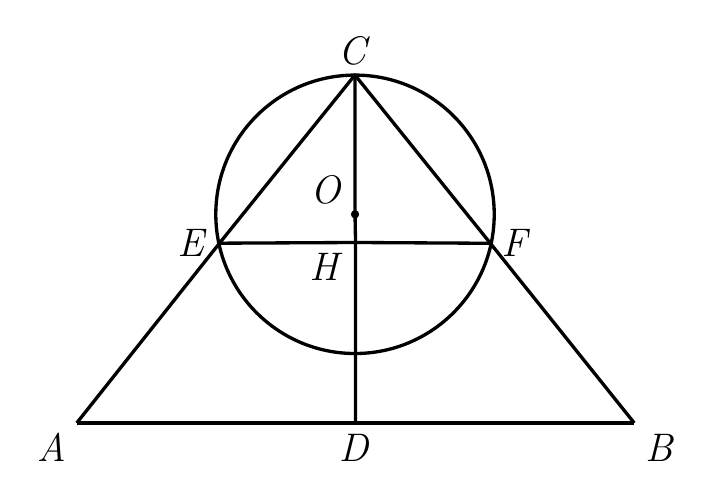
\begin{tikzpicture}[line width=1.2pt, line join=round]
\coordinate (A) at (-3.556,-2.202);
\coordinate (B) at (3.524,-2.202);
\coordinate (C) at (-0.023,2.217);
\coordinate (D) at (-0.015,-2.202);
\coordinate (E) at (-1.743,0.081);
\coordinate (F) at (1.697,0.080);
\coordinate (H) at (-0.015,0.090);
\coordinate (O) at (-0.022,0.448);




\draw (O) circle (1.768);


\draw (A) -- (E) -- (C) -- (F) -- (B);


\draw (A) -- (D) -- (B);


\draw (C) -- (O) -- (H) -- (D);


\draw (E) -- (H) -- (F);


\fill (O) circle (1.500pt);


\node[above, font=\fontsize{14}{16.8}\selectfont] at (C) {$\mathit{C}$};
\node[left, font=\fontsize{14}{16.8}\selectfont] at (E) {$\mathit{E}$};
\node[right, font=\fontsize{14}{16.8}\selectfont] at (F) {$\mathit{F}$};
\node[below left, font=\fontsize{14}{16.8}\selectfont] at (H) {$\mathit{H}$};
\node[above left, font=\fontsize{14}{16.8}\selectfont] at (O) {$\mathit{O}$};
\node[below left, font=\fontsize{14}{16.8}\selectfont] at (A) {$\mathit{A}$};
\node[below right, font=\fontsize{14}{16.8}\selectfont] at (B) {$\mathit{B}$};
\node[below, font=\fontsize{14}{16.8}\selectfont] at (D) {$\mathit{D}$};
\end{tikzpicture}
\end{document}